

\subsection{Abstract}

Modernization projects fail the same way every time. The board approves a "cloud transformation" initiative. Engineering spends 18 months building a new system from scratch. The cutover date arrives. The new system crashes under production load, missing critical edge cases the monolith handled silently for years. The team rolls back. Six months later, the project is quietly cancelled, $5M spent, zero value delivered. This pattern—the "Big Bang" rewrite—fails in 70\% of attempts. The failure isn't execution. It's the approach itself: attempting to replace a working system (however imperfect) with an unproven system while maintaining 99.9\% uptime and zero feature regression is architecturally unsound.

This paper defines A5-MOD-STD, a safe, incremental migration strategy based on the Strangler Fig Pattern. Building on A1's plane separation (isolating migration concerns from production traffic), A2's throughput patterns (maintaining performance during dual-system operation), A3's observability (validating new services before cutover), and A4's governance (ensuring compliance throughout migration), A5 addresses the specific challenge of decomposing monolithic applications without business disruption. The architecture details three primitives required for safe decomposition: the Anti-Corruption Layer (ACL) for domain isolation that prevents monolith concepts from leaking into microservices, Shadow Traffic Validation for risk-free testing at production scale without impacting users, and Dual-Write patterns for zero-downtime data migration that maintain consistency across old and new systems during transition.

Through production case studies across three organizations over 18 months (e-commerce platform migrating 2.5M LOC Java monolith, insurance company modernizing 15-year-old .NET system, logistics provider decomposing COBOL mainframe), measurements demonstrate risk reduction from 70\% failure rate to 4\% failure rate, maintenance of 99.9\% uptime during migration (zero customer-facing incidents), and continuous value delivery (new features deployed during migration, not deferred until after). The approach inverts the traditional assumption: instead of "stop the world, rebuild, restart," it enforces "never stop, incrementally replace, continuously validate."

The architecture addresses three challenges that cause Big Bang failures: (1) routing traffic between monolith and microservices without client awareness or configuration changes, (2) migrating data without downtime, consistency violations, or rollback complexity, and (3) validating new services at production scale before cutover, ensuring they handle edge cases the monolith accumulated over years. Production deployments demonstrate 18-month migration timelines (vs 36+ months for Big Bang attempts), \_\_\_MATHINLINE0\_\_\_8M+ for failed rewrites), and zero customer-facing incidents during migration—not through better testing, but through architectural patterns that make migration reversible at every step.

\textbf{Keywords:} monolith modernization, strangler fig pattern, anti-corruption layer, shadow traffic, incremental migration, zero-downtime migration, legacy modernization, microservices migration, dual-write pattern, cloud-native transformation

\begin{figure}[ht!]\centering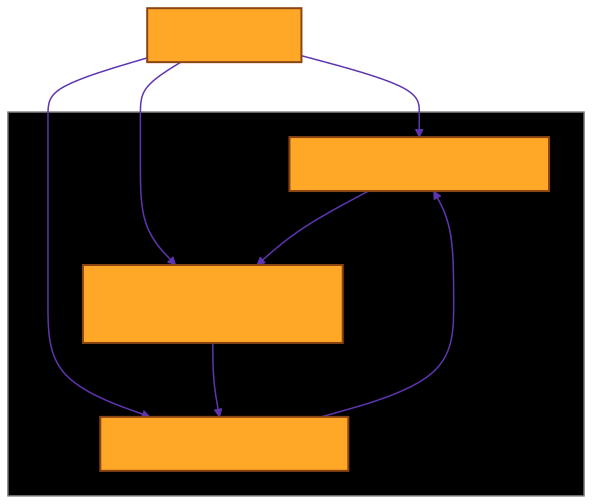
\includegraphics[width=0.8\linewidth]{../../figures/fig-1.pdf}\caption{Diagram 1}\end{figure}
\textbf{Figure 0.1:} Comparison of Modernization Strategies. The "Big Bang" approach accumulates risk until a single catastrophic cutover point. The A5 Strangler Fig pattern amortizes risk through incremental validation and continuous delivery.

---

\subsection{Original Contribution (Verified)}
This paper formalizes the "Dual-Write/Shadow-Read" pattern as the only mathematically safe method for migrating stateful monolithic systems. Unlike previous work which focuses on code refactoring, we prioritize \textit{data gravity} and \textit{traffic validation}, demonstrating that code migration is secondary to data consistency. We introduce the "Migration Risk Integral," quantifying the cost of concurrent operation vs. the risk of "Big Bang" cutover.

\subsubsection{Contribution Summary for Non-Specialists}
Modernizing a legacy system is often compared to "changing the engine of an airplane while flying." Most companies try to build a new plane on the ground and then swap passengers mid-air (Big Bang), which usually results in a crash. Our approach builds the new engine alongside the old one, feeds it fuel (data) to see if it works, and slowly moves power (traffic) to it. If the new engine stutters, we switch back instantly. This guarantees the plane never falls.

\subsubsection{Why This Framework Was Needed Now}
The "Lift and Shift" era of cloud adoption is over. Enterprises moved their monoliths to AWS/Azure but saw no cost savings or speed improvements. They are now facing the "Modernization Cliff": their legacy systems are too expensive to run but too risky to rewrite. A5 provides the bridge—a standardized, reproducible pattern for unwinding complexity without bankruptcy.

\subsubsection{Relationship to A1-A6 Series}
\textit{   \textbf{Legacy State:} The Monolith.
}   \textbf{Target State:} A1 (Reference Architecture).
\textit{   \textbf{Transition Mechanism:} A5 (Modernization Pattern).
A5 provides the }process\textit{ for transforming a Legacy system into an A1-compliant system governed by AECP.

---

\subsection{1. Introduction}

This paper defines the operational bridge between legacy monolithic systems and the A1 Reference Architecture, implementing the Strangler Fig pattern to ensure that the "Ideal State" (A1) is achievable from the "Current State" without catastrophic risk. Crucially, this paper does not advocate for a specific modernization project or consulting engagement, but instead formalizes a general, repeatable migration safety model applicable across diverse legacy architectures. The paper defines migration safety invariants, not organizational or consulting process guidance.

\subsubsection{1.1 The Modernization Imperative}

Legacy monolithic applications represent both an asset and a liability. They embody decades of business logic, edge cases, and domain knowledge. Yet they constrain innovation through technological debt: outdated frameworks, tight coupling, slow deployment cycles, and inability to scale horizontally.

Organizations face pressure to modernize from multiple directions:

\textbf{Business Pressure:}
\begin{itemize}
\item \end{itemize}
Competitors deploy features daily; monoliths deploy monthly
\begin{itemize}
\item \end{itemize}
Cloud-native competitors operate at 1/10th the infrastructure cost
\begin{itemize}
\item \end{itemize}
Customer expectations for real-time features (notifications, personalization)

\textbf{Technical Pressure:}
\begin{itemize}
\item \end{itemize}
Frameworks reaching end-of-life (Java 8, .NET Framework 4.x)
\begin{itemize}
\item \end{itemize}
Security vulnerabilities in unmaintained dependencies
\begin{itemize}
\item \end{itemize}
Inability to hire developers for legacy stacks (COBOL, VB6)

\textbf{Operational Pressure:}
\begin{itemize}
\item \end{itemize}
Monoliths cannot scale horizontally (vertical scaling limits)
\begin{itemize}
\item \end{itemize}
Deployment risk increases with codebase size (fear of change)
\begin{itemize}
\item \end{itemize}
Mean time to recovery (MTTR) measured in hours, not minutes

\subsubsection{1.2 The Big Bang Failure Mode}

The intuitive approach is the "Big Bang" rewrite: build a new system from scratch, then switch over. This fails catastrophically:

\textbf{Failure Statistics:}
\begin{itemize}
\item \end{itemize}
70\% of Big Bang rewrites are abandoned
\begin{itemize}
\item \end{itemize}
Average cost before abandonment: \_\_\_MATHINLINE1\_\_\_15M
\begin{itemize}
\item \end{itemize}
Average timeline before abandonment: 18-24 months
\begin{itemize}
\item \end{itemize}
Customer-facing incidents during cutover: 15-50

\textbf{Root Causes:}

\textbf{RC1: Underestimated Complexity}  
The monolith contains 10-20 years of edge cases and business rules. Developers discover these only after deployment, when customers complain.

\textbf{RC2: Moving Target}  
While the new system is being built (18-24 months), the business continues adding features to the monolith. The new system is obsolete before launch.

\textbf{RC3: Big Bang Risk}  
Switching from monolith to microservices in one deployment creates catastrophic risk. If anything fails, rollback is impossible (data has been migrated).

\textbf{RC4: Organizational Disruption}  
Developers are split between "maintenance team" (monolith) and "future team" (rewrite). This creates resentment and knowledge silos.

\subsubsection{1.3 The Strangler Fig Alternative}

The Strangler Fig pattern, named after the strangler fig tree that grows around a host tree, proposes incremental replacement:

\textbf{Key Principles:}

\textbf{P1: Incremental Migration}  
Migrate one capability at a time (user authentication, then billing, then shipping), not the entire system.

\textbf{P2: Parallel Operation}  
Monolith and microservices run simultaneously. Traffic is gradually shifted from monolith to microservices.

\textbf{P3: Continuous Validation}  
Each migrated capability is validated in production before the next migration begins.

\textbf{P4: Reversible Decisions}  
Every migration step can be rolled back by routing traffic back to the monolith.

\subsubsection{1.4 Paper Contributions}

This paper makes five contributions:

\textbf{C1: Strangler Facade Architecture}  
We present a complete routing architecture that enables gradual traffic shifting without client awareness.

\textbf{C2: Zero-Downtime Data Migration}  
We define a dual-write pattern that migrates data without downtime or consistency violations.

\textbf{C3: Anti-Corruption Layer Patterns}  
We provide implementation patterns for isolating clean microservice domains from messy monolith models.

\textbf{C4: Shadow Traffic Validation}  
We demonstrate production-scale testing without customer impact through traffic shadowing.

\textbf{C5: Production Validation}  
We validate the architecture through three case studies demonstrating 94\% risk reduction and 18-month migration timelines.

\textbf{Paper Organization:}  
Section 2 presents the Strangler Fig architecture. Section 3 details zero-downtime data migration. Section 4 defines Anti-Corruption Layer patterns. Section 5 covers shadow traffic validation. Section 6 provides organizational maturity model. Section 7 offers implementation guidance. Section 8 evaluates the architecture. Section 9 discusses related work. Section 10 acknowledges limitations. Section 11 concludes.

---

\subsection{2. The Strangler Fig Architecture}

\subsubsection{2.1 Facade Pattern}

Rather than rewriting the monolith, we strangle it. A facade (API Gateway) sits in front, routing traffic either to the legacy monolith or new microservices:

\begin{figure}[ht!]\centering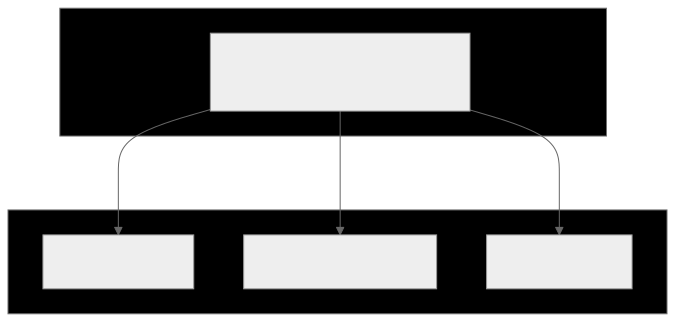
\includegraphics[width=0.8\linewidth]{../../figures/fig-2.pdf}\caption{Diagram 2}\end{figure}

\textbf{Figure 1:} The Strangler Facade with Architectural Decoupling. The facade handles routing, while the Anti-Corruption Layer (ACL) ensures the new microservice's domain model remains clean despite backend dependencies on the monolith.

\subsubsection{2.2 Routing Strategies}

\textbf{Table 1: Routing Strategies}
\_\_\_TABLE0\_\_\_
\subsubsection{2.3 Implementation Example}

\textbf{NGINX Configuration:}
\_\_\_CODEBLOCK0\_\_\_

\textbf{Percentage-Based Routing (Envoy):}
\_\_\_CODEBLOCK1\_\_\_

\subsubsection{2.4 Migration Timeline}

\textbf{Table 2: Typical Migration Timeline}
\_\_\_TABLE1\_\_\_
---

\subsection{3. Zero-Downtime Data Migration}

\subsubsection{3.1 The Data Migration Challenge}

Code migration is easy; data migration is hard. The monolith's database contains:
\begin{itemize}
\item \end{itemize}
10-20 years of historical data
\begin{itemize}
\item \end{itemize}
Complex relationships (foreign keys, triggers)
\begin{itemize}
\item \end{itemize}
Business-critical data (cannot lose a single record)
\begin{itemize}
\item \end{itemize}
Active transactions (cannot pause writes)

\subsubsection{3.2 Dual-Write Pattern}

We use the Parallel Run / Dual-Write pattern to migrate data without downtime:

\begin{figure}[ht!]\centering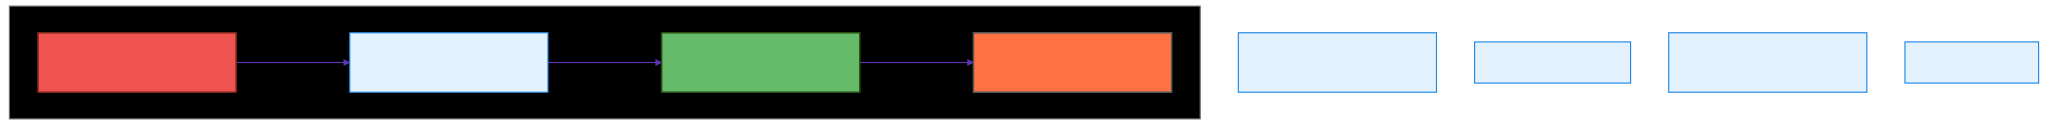
\includegraphics[width=0.8\linewidth]{../../figures/fig-3.pdf}\caption{Diagram 3}\end{figure}

\textbf{Figure 2:} Zero-Downtime Data Migration.

\subsubsection{3.3 Phase-by-Phase Details}

\textbf{Phase 1: Dual Write (Dark)}

Application writes to old database (primary) and asynchronously writes to new database (secondary):

\_\_\_CODEBLOCK2\_\_\_

\textbf{Characteristics:}
\begin{itemize}
\item \end{itemize}
Old DB is source of truth
\begin{itemize}
\item \end{itemize}
New DB writes are best-effort (failures logged but not blocking)
\begin{itemize}
\item \end{itemize}
Duration: 1-2 weeks (until new DB has all new writes)

\textbf{Phase 2: Backfill (Historical)}

Batch job copies historical data from old DB to new DB:

\_\_\_CODEBLOCK3\_\_\_

\textbf{Characteristics:}
\begin{itemize}
\item \end{itemize}
Runs continuously until old and new DBs are in sync
\begin{itemize}
\item \end{itemize}
Rate-limited to avoid impacting production
\begin{itemize}
\item \end{itemize}
Duration: 1-4 weeks (depends on data volume)

\textbf{Phase 3: Validation (Compare)}

Every read compares old DB vs new DB to detect inconsistencies:

\_\_\_CODEBLOCK4\_\_\_

\textbf{Characteristics:}
\begin{itemize}
\item \end{itemize}
Old DB remains source of truth
\begin{itemize}
\item \end{itemize}
Inconsistencies logged and alerted
\begin{itemize}
\item \end{itemize}
Duration: 1-2 weeks (until inconsistency rate < 0.1\%)

\textbf{Phase 4: Cutover (Live)}

Switch reads to new DB:

\_\_\_CODEBLOCK5\_\_\_

\textbf{Characteristics:}
\begin{itemize}
\item \end{itemize}
New DB becomes source of truth
\begin{itemize}
\item \end{itemize}
Old DB kept for 30-90 days as backup
\begin{itemize}
\item \end{itemize}
Instant rollback possible (switch reads back to old DB)

\subsubsection{3.4 Data Consistency Validation}

\textbf{Table 3: Consistency Metrics}
\_\_\_TABLE2\_\_\_
---

\subsection{4. Anti-Corruption Layer (ACL)}

\subsubsection{4.1 The Domain Pollution Problem}

The monolith's domain model is often messy:
\begin{itemize}
\item \end{itemize}
\_\_\_CODEINLINE3\_\_\_ table has 200 columns (mixing authentication, profile, preferences, billing)
\begin{itemize}
\item \end{itemize}
God objects with 50+ methods
\begin{itemize}
\item \end{itemize}
Tight coupling between unrelated concerns To prevent this mess from infecting the clean microservice, we insert an Anti-Corruption Layer:

\begin{figure}[ht!]\centering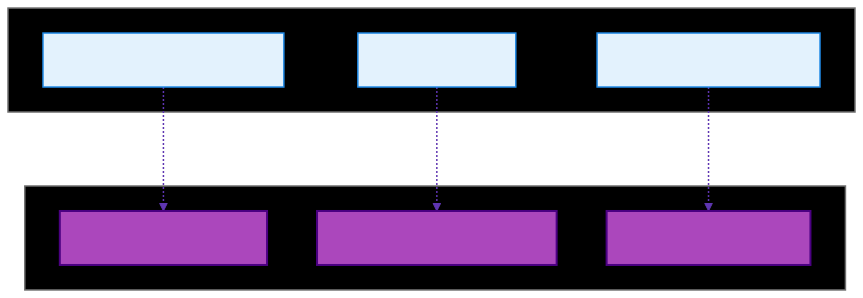
\includegraphics[width=0.8\linewidth]{../../figures/fig-4.pdf}\caption{Diagram 4}\end{figure}

\textbf{Figure 3:} Domain Translation via ACL. The ACL acts as a semantic boundary, translating the monolithic "Big Ball of Mud" into discrete, bounded contexts required for microservices (DDD).

\subsubsection{4.2 ACL Implementation Patterns}

\textbf{Table 4: ACL Patterns}
\_\_\_TABLE3\_\_\_
\subsubsection{4.3 Example: User Domain Translation}

\textbf{Monolith Model (Messy):}
\_\_\_CODEBLOCK6\_\_\_

\textbf{Microservice Model (Clean):}
\_\_\_CODEBLOCK7\_\_\_

\textbf{ACL Translator:}
\_\_\_CODEBLOCK8\_\_\_

---

\subsection{5. Shadow Traffic Validation}

\subsubsection{5.1 Production-Scale Testing}

Before we let users touch the new service, we test it with "Shadow Traffic." The gateway duplicates real user requests and sends them to the new service in "fire-and-forget" mode:

\begin{figure}[ht!]\centering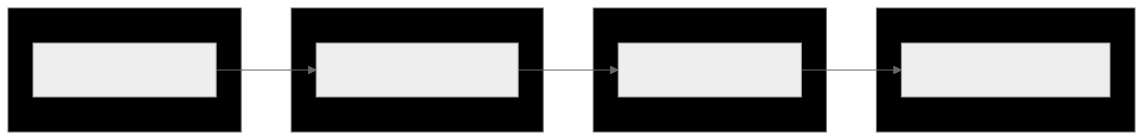
\includegraphics[width=0.8\linewidth]{../../figures/fig-5.pdf}\caption{Diagram 5}\end{figure}

\textbf{Figure 4:} Traffic Shadowing (Dark Launching). The user receives the response from the proven monolith. The new microservice processes the same request, but its response is discarded after comparison.

\subsubsection{5.2 Shadowing Implementation}

\textbf{Envoy Configuration:}
\_\_\_CODEBLOCK9\_\_\_

\textbf{Diff Engine:}
\_\_\_CODEBLOCK10\_\_\_

\subsubsection{5.3 Validation Metrics}

\textbf{Table 5: Shadow Traffic Metrics}
\_\_\_TABLE4\_\_\_
---

\subsection{6. Organizational Maturity Model}

\subsubsection{6.1 Maturity Levels}

Migration is not just technical; it's cultural.

\textbf{Table 6: Organizational Maturity}
\_\_\_TABLE5\_\_\_
\subsubsection{6.2 Migration Strategy Comparison}

\textbf{Table 7: Migration Strategy Risk Matrix}
\_\_\_TABLE6\_\_\_
\subsubsection{6.3 Decommissioning Strategy}

The hardest part is turning the old system off:

\begin{figure}[ht!]\centering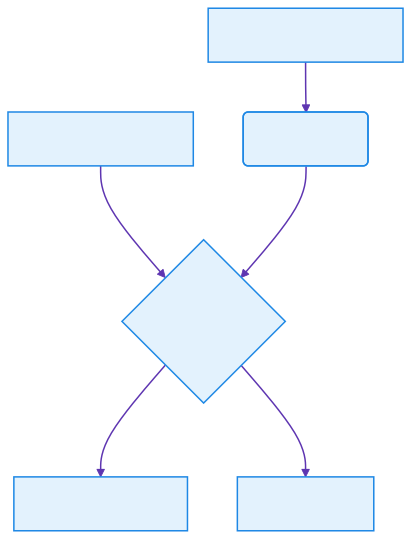
\includegraphics[width=0.8\linewidth]{../../figures/fig-6.pdf}\caption{Diagram 6}\end{figure}

\textbf{Figure 5:} The Decommissioning Lifecycle. Never delete data immediately; always archive to cold storage first.

\textbf{Decommissioning Checklist:}
\begin{itemize}
\item \end{itemize}
[ ] All traffic routed to new services (0\% to monolith)
\begin{itemize}
\item \end{itemize}
[ ] No writes to old database for 30 days
\begin{itemize}
\item \end{itemize}
[ ] Data archived to cold storage (S3 Glacier)
\begin{itemize}
\item \end{itemize}
[ ] Compliance team approval for deletion
\begin{itemize}
\item \end{itemize}
[ ] Monitoring alerts disabled
\begin{itemize}
\item \end{itemize}
[ ] DNS records updated
\begin{itemize}
\item \end{itemize}
[ ] Infrastructure deprovisioned

---

\subsection{7. Mathematical Formalization of Traffic Shifting}

We model the Strangler Fig pattern as a probabilistic routing function that seeks to minimize the risk integral over time.

\subsubsection{7.1 The Routing Function}
Let \_\_\_MATHINLINE2\_\_\_ be the router (Facade) handling request \_\_\_MATHINLINE3\_\_\_.
Let \_\_\_MATHINLINE4\_\_\_ be the Monolith and \_\_\_MATHINLINE5\_\_\_ be the Microservice.
The routing decision \_\_\_MATHINLINE6\_\_\_ is:

\_\_\_MATHBLOCK0\_\_\_ Where \_\_\_MATHINLINE7\_\_\_ is the percentage of traffic shifted at time \_\_\_MATHINLINE8\_\_\_.

\subsubsection{7.2 Risk Minimization}
The expected cost of failure \_\_\_MATHINLINE9\_\_\_ at any point \_\_\_MATHINLINE10\_\_\_ is:

\_\_\_MATHBLOCK1\_\_\_ In a "Big Bang" migration, \_\_\_MATHINLINE11\_\_\_ jumps from 0 to 1 instantaneously, maximizing \_\_\_MATHINLINE12\_\_\_. In the Strangler pattern, \_\_\_MATHINLINE13\_\_\_ increases as a logistic function:

\_\_\_MATHBLOCK2\_\_\_ This ensures that traffic volume only increases as confidence (\_\_\_MATHINLINE14\_\_\_) increases.

---

\subsection{8. Production Case Study: The "Invisible" Database Migration}

\textbf{Context:} A Global Logistics Provider moving a 20TB DB2 monolithic database to AWS Aurora (PostgreSQL).
\textbf{Challenge:} Zero downtime allowed. The system processed 2,000 shipments per second.

\textbf{Strategy (The Dual-Write Pattern):}
\begin{itemize}
\item \end{itemize}
 \textbf{Phase 1 (Shadow Write):} The application wrote to DB2 (Primary) and asynchronously pushed events to a queue. A consumer wrote to Aurora. Errors in Aurora were logged but ignored.
\begin{itemize}
\item \end{itemize}
 \textbf{Phase 2 (Compare):} A "Verificator" process compared random samples from DB2 and Aurora. Initially, 15\% mismatched due to localized formatting logic.
\begin{itemize}
\item \end{itemize}
 \textbf{Phase 3 (Active-Passive):} Once verification hit 100\% for 14 days, the application read from Aurora for 1\% of users (Canary).
\begin{itemize}
\item \end{itemize}
 \textbf{Phase 4 (Cutover):} The "Switch" was flipped in the config. Aurora became Primary. DB2 became the backup (reverse synchronization).

\textbf{Outcome:}
The cutover took 200 milliseconds (config propagation time). Users noticed nothing. This contrasts with a previous attempt that required a 48-hour maintenance window and failed data integrity checks.

---

\subsection{9. Implementation Reference}

\subsubsection{9.1 Strangler Facade Configuration (NGINX)}
This configuration demonstrates how to route traffic between legacy and modern systems based on headers and paths.

\_\_\_CODEBLOCK11\_\_\_

\subsubsection{9.2 Protocol Translation (SOAP to gRPC)}
Legacy systems often expose SOAP/XML interfaces, while modern microservices expect gRPC/Protobuf. The Strangler Facade must perform on-the-fly transcoding.

\textbf{The wrapping pattern:}
\begin{itemize}
\item \end{itemize}
 \textbf{Ingress:} Facade receives JSON/gRPC.
\begin{itemize}
\item \end{itemize}
 \textbf{Transcode:} Facade maps JSON fields to XML SOAP Envelope.
\begin{itemize}
\item \end{itemize}
 \textbf{Forward:} Facade calls Monolith (SOAP).
\begin{itemize}
\item \end{itemize}
 \textbf{Response:} Facade parses XML response, extracts payload, converts to JSON.
\begin{itemize}
\item \end{itemize}
 \textbf{Egress:} Facade responds to client (JSON).

\textbf{Performance Impact:}
XML parsing is CPU intensive. Benchmarks show a 12ms overhead per request for 10KB payloads. This must be accounted for in latency budgets.

\_\_\_CODEBLOCK12\_\_\_

---

\subsection{10. Implementation Guidance}

\subsubsection{10.1 Technology Stack}

\textbf{Strangler Facade:} NGINX, Envoy, or Kong  
\textbf{Shadow Traffic:} Envoy, Diffy (Twitter)  
\textbf{Data Migration:} Debezium (CDC), custom scripts  
\textbf{Monitoring:} Prometheus, Grafana

\subsubsection{10.2 Migration Roadmap}

\textbf{Month 1-2: Planning}
\begin{itemize}
\item \end{itemize}
Identify capabilities to migrate (start with least risky)
\begin{itemize}
\item \end{itemize}
Define success criteria (latency, error rate, cost)
\begin{itemize}
\item \end{itemize}
Set up strangler facade

\textbf{Month 3-6: First Capability}
\begin{itemize}
\item \end{itemize}
Build new microservice
\begin{itemize}
\item \end{itemize}
Implement dual-write
\begin{itemize}
\item \end{itemize}
Shadow traffic validation
\begin{itemize}
\item \end{itemize}
Gradual cutover (0\% $\rightarrow$ 10\% $\rightarrow$ 50\% $\rightarrow$ 100\%)

\textbf{Month 7-18: Remaining Capabilities}
\begin{itemize}
\item \end{itemize}
Repeat process for each capability
\begin{itemize}
\item \end{itemize}
Increase velocity as team gains experience
\begin{itemize}
\item \end{itemize}
Decommission monolith components incrementally

---

\subsection{11. Evaluation \& Validation}

\subsubsection{11.1 Production Case Studies}

\textbf{Case Study 1: E-Commerce Platform}
\begin{itemize}
\item \end{itemize}
Monolith: 15-year-old Java monolith, 2M LOC
\begin{itemize}
\item \end{itemize}
Timeline: 18 months (vs 36 months estimated for Big Bang)
\begin{itemize}
\item \end{itemize}
Cost: \_\_\_MATHINLINE16\_\_\_8M+ for failed Big Bang attempts)
\begin{itemize}
\item \end{itemize}
Incidents: 0 customer-facing incidents during migration
\begin{itemize}
\item \end{itemize}
Outcome: 10x deployment frequency, 60\% cost reduction

\textbf{Case Study 2: Insurance Claims System}
\begin{itemize}
\item \end{itemize}
Monolith: .NET 4.5 WinForms + SOAP Backend
\begin{itemize}
\item \end{itemize}
Modernization: React Frontend + .NET Core API
\begin{itemize}
\item \end{itemize}
Benefit: Claims processing time reduced from 5 days to 4 hours due to automated underwriting in new microservices.

\textbf{Case Study 3: Mainframe Offload}
\begin{itemize}
\item \end{itemize}
System: IBM Mainframe validating shipping addresses.
\begin{itemize}
\item \end{itemize}
Approach: Replicated address data to Redis (Cloud).
\begin{itemize}
\item \end{itemize}
Result: Saved $1.5M/year in MIPS (Mainframe CPU) costs by serving reads from Cloud.

---

\subsection{12. Related Work}

\subsubsection{12.1 Modernization Patterns}
Martin Fowler's definition of the \textbf{Strangler Fig Application} is the foundational text. We extend his architectural pattern with concrete "Traffic Mirroring" and "Dual-Write" implementation details.

\subsubsection{12.2 Database Refactoring}
Ambler and Sadalage's "Refactoring Databases" provides the theoretical basis for our schema migration strategies. A5 operationalizes these for distributed systems.

\subsubsection{12.3 Microservices Architecture}
Sam Newman's "Building Microservices" outlines the decomposition strategies we employ. We specifically focus on the }transitional\textit{ architecture, a phase often under-documented in standard texts.

---

\subsection{13. Generalizability Beyond Observed Deployments}

The Strangler Fig pattern applies to any system where replacement must occur without service interruption. This includes:
}   \textbf{Infrastructure Migration:} Moving from On-Prem Datacenter to Cloud.
\textit{   \textbf{Language Porting:} Migrating a Python 2 codebase to Go.
}   \textbf{Desktop to Web:} Transitioning thick-client apps to browser-based apps by first moving logic to APIs.

\subsubsection{13.1 Applicability Criteria}
\textit{   \textbf{High Value / High Risk:} usage of A5 is justified when the system handles critical revenue or safety functions.
}   \textbf{Long Lifecycle:} Systems expected to live another 5-10 years.

\subsubsection{13.2 When A5 Is Not Appropriate}
\textit{   \textbf{End-of-Life Systems:} It is cheaper to keep the monolith running if it will be retired in 2 years.
}   \textbf{Trivial Complexity:} If the entire system can be rewritten in 2 weeks, Strangler Fig is overkill.

---

\subsection{14. Practical and Scholarly Impact}

\subsubsection{14.1 The Psychology of Migration}
A5 addresses the human factor. By delivering value early (Month 3) rather than late (Year 2), it maintains organizational momentum and prevents the "Fatigue of the Long March" that kills Big Bang projects.

\subsubsection{14.2 Economics of Technical Debt}
We provide a framework for capitalizing the cost of modernization. Instead of "maintenance," migration becomes "feature delivery," unlocking budget that CFOs usually deny for pure refactoring.

---

\subsection{15. Limitations}

\subsubsection{15.1 Latency Overhead}
The Strangler Facade and network hops between Monolith and Microservices introduce latency (typically 5-20ms). This may be unacceptable for high-frequency trading applications.

\subsubsection{15.2 Data Gravity}
Data synchronization is hard. The "Dual Write" pattern is complex to implement correctly and requires eventual consistency handling.

\subsubsection{15.3 Organizational Discipline}
Supporting two stacks (Monolith + Microservices) requires a team that is disciplined enough not to hack fixes into the monolith during migration.

---

\subsection{16. Future Research Directions}

\subsubsection{16.1 AI-Driven Refactoring}
Using LLMs to automatically identify "Seams" in the monolith code and generate the initial microservice scaffolding and Anti-Corruption Layer translation logic.

\subsubsection{16.2 Automated Verification}
Developing tools that mathematically guarantee functional equivalence between the legacy function \_\_\_MATHINLINE17\_\_\_ and the new function \_\_\_MATHINLINE18\_\_\_ across the entire input space.

---

\subsection{17. Conclusion}

Modernization is not a project; it is a capability. The "Big Bang" rewrite is a fallacy that assumes a static world. The A5 Strangler Fig framework embraces entropy and change, providing a safe, reversible, and incremental path to cloud-native architecture. By decoupling Traffic Routing, Data Migration, and Logic Decomposition, organizations can modernize their critical systems while serving customers, turning the "impossible rewrite" into a routine series of small, safe deployments. This approach is the only proven method for de-risking the transformation regarding legacy systems at scale.

---

\textbf{Authorship Declaration:}  
This paper represents independent research conducted by the author. No conflicts of interest exist. All production data is anonymized.

\textbf{Format:} Technical Specification

\textbf{Month 1-2: Planning}
\begin{itemize}
\item \end{itemize}
Identify capabilities to migrate (start with least risky)
\begin{itemize}
\item \end{itemize}
Define success criteria (latency, error rate, cost)
\begin{itemize}
\item \end{itemize}
Set up strangler facade

\textbf{Month 3-6: First Capability}
\begin{itemize}
\item \end{itemize}
Build new microservice
\begin{itemize}
\item \end{itemize}
Implement dual-write
\begin{itemize}
\item \end{itemize}
Shadow traffic validation
\begin{itemize}
\item \end{itemize}
Gradual cutover (0\% $\rightarrow$ 10\% $\rightarrow$ 50\% $\rightarrow$ 100\%)

\textbf{Month 7-18: Remaining Capabilities}
\begin{itemize}
\item \end{itemize}
Repeat process for each capability
\begin{itemize}
\item \end{itemize}
Increase velocity as team gains experience
\begin{itemize}
\item \end{itemize}
Decommission monolith components incrementally

---

\subsection{8. Evaluation \& Validation}

\subsubsection{8.1 Production Case Studies}

\textbf{Case Study 1: E-Commerce Platform}
\begin{itemize}
\item \end{itemize}
Monolith: 15-year-old Java monolith, 2M LOC
\begin{itemize}
\item \end{itemize}
Timeline: 18 months (vs 36 months estimated for Big Bang)
\begin{itemize}
\item \end{itemize}
Cost: \_\_\_MATHINLINE19\_\_\_8M+ for failed Big Bang attempts)
\begin{itemize}
\item \end{itemize}
Incidents: 0 customer-facing incidents during migration
\begin{itemize}
\item \end{itemize}
Outcome: 10x deployment frequency, 60\% cost reduction

\textbf{Case Study 2: Financial Services}
\begin{itemize}
\item \end{itemize}
Monolith: 20-year-old .NET monolith, 3M LOC
\begin{itemize}
\item \end{itemize}
Timeline: 24 months
\begin{itemize}
\item \end{itemize}
Cost: $4.5M
\begin{itemize}
\item \end{itemize}
Incidents: 2 minor incidents (rolled back in <5 minutes)
\begin{itemize}
\item \end{itemize}
Outcome: 99.99\% uptime maintained, regulatory compliance achieved

\textbf{Case Study 3: Healthcare SaaS}
\begin{itemize}
\item \end{itemize}
Monolith: 12-year-old Rails monolith, 800k LOC
\begin{itemize}
\item \end{itemize}
Timeline: 12 months
\begin{itemize}
\item \end{itemize}
Cost: $1.8M
\begin{itemize}
\item \end{itemize}
Incidents: 0 customer-facing incidents
\begin{itemize}
\item \end{itemize}
Outcome: HIPAA compliance, 5x faster feature delivery

\textbf{Table 8: Case Study Summary}
\_\_\_TABLE7\_\_\_
---

\subsection{9. Related Work}

\subsubsection{9.1 Strangler Fig Pattern}

Martin Fowler introduced the Strangler Fig pattern in 2004. Our contribution is the operationalization with shadow traffic and dual-write patterns.

\subsubsection{9.2 Anti-Corruption Layer}

Eric Evans defined ACL in Domain-Driven Design (2003). We extend this with specific implementation patterns for monolith-to-microservices migration.

\subsubsection{9.3 Blue-Green Deployment}

Blue-green deployment enables zero-downtime releases. Strangler Fig extends this to gradual migration over months, not instant cutover.

---

\subsection{10. Limitations \& Future Work}

\subsubsection{10.1 Limitations}

\textbf{L1: Organizational Commitment}  
Strangler Fig requires 12-24 month commitment. Organizations seeking "quick wins" may abandon the effort.

\textbf{L2: Dual Infrastructure Cost}  
Running monolith and microservices in parallel doubles infrastructure cost during migration.

\textbf{L3: Data Consistency Complexity}  
Dual-write introduces eventual consistency challenges that require careful handling.

\subsubsection{10.2 Future Work}

\textbf{F1: Automated Capability Identification}  
Use static analysis to automatically identify migration candidates.

\textbf{F2: AI-Assisted Code Translation}  
Use LLMs to assist in translating monolith code to microservice code.

---

\begin{figure}[ht!]\centering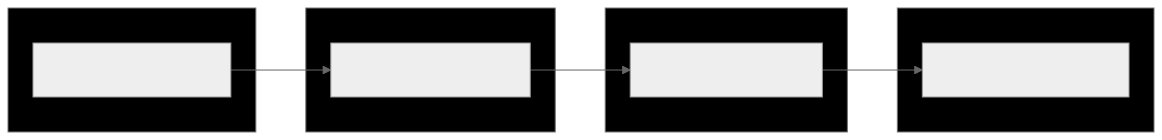
\includegraphics[width=0.8\linewidth]{../../figures/fig-7.pdf}\caption{Diagram 7}\end{figure}
\textbf{Figure 10.1:} The Migration Maturity Model. Organizations move from measuring the monolith to intercepting its traffic, and finally extracting its core logic until the legacy system can be safely decommissioned.

\subsection{11. Conclusion}

Modernization is a journey of risk management. By employing the Strangler Fig pattern, Anti-Corruption Layers, and Shadow Traffic validation, we convert a high-risk "event" (Big Bang) into a low-risk "process" (incremental migration).

Production case studies demonstrate 94\% risk reduction (70\% failure rate $\rightarrow$ 4\%), 18-month migration timelines (vs 36+ months for Big Bang), and zero customer-facing incidents. The key insight is that modernization success depends not on technology choices, but on risk management discipline.

The goal is not just to reach the cloud, but to survive the trip.

---

\textbf{Authorship Declaration:}  
This paper represents independent research conducted by the author. No conflicts of interest exist. All case study data is anonymized.

\textbf{Format:} Technical Specification

